% 11_defects
\section{Localized defects}\label{sec:defects}

\Cref{asm:closure} posits a pressureless product carrying a fraction $\bfrac$
of the converted energy. This section asks what such an object could be. The
answer offered is a topological texture, and the section is careful about what
is and is not established: a finite-energy solution with an integer charge and
a preferred size is exhibited and solved, but its identification with dark
matter remains a conjecture, and its abundance is not computed.

\subsection{An obstruction, and how to evade it}\label{sec:defects-derrick}

\begin{proposition}[Derrick scaling]\label{prop:derrick}
  In three spatial dimensions let $E[\phi]=E_2+E_0$ with
  $E_2=\tfrac12\int|\nabla\phi|^2$ and $E_0=\int W(\phi)$, both finite and
  $W\ge0$ after subtracting the vacuum. Under $\phi_\sigma(\mathbf
  x)=\phi(\sigma\mathbf x)$ one has $E(\sigma)=\sigma^{-1}E_2+\sigma^{-3}E_0$,
  so a non-trivial stationary point would require $E_2+3E_0=0$, impossible for
  $E_2>0$.
\end{proposition}

A single static canonical scalar therefore has no stable localized solution.
The hypotheses are what matter: time dependence, a conserved charge, gauge
fields, gravity, or additional terms in the energy each evade the conclusion.
We take the last route. Let $n^A(\mathbf x)$, $A=1,\dots,4$, satisfy
$n^An^A=1$ with a constant value at infinity, so that configurations are maps
$S^3\to S^3$, and take
%
\begin{equation}\label{eq:defects-energy}
  E=\int \dd^3x\left[\frac{\Fstar^2}{2}\partial_i n^A\partial_i n^A
  +\frac{\kaps}{4}\mathcal W_{ij}^{AB}\mathcal W_{ij}^{AB}\right],
  \qquad
  \mathcal W_{ij}^{AB}=\partial_i n^A\partial_j n^B-\partial_j n^A\partial_i n^B ,
\end{equation}
%
with $\Fstar>0$ of mass dimension one and $\kaps>0$ dimensionless. Under the
same scaling the two terms go as $\sigma^{-1}$ and $\sigma^{+1}$, so
\cref{prop:derrick} no longer applies and a preferred size exists. This is the
Skyrme mechanism, and \cref{eq:defects-energy} is the $\mathrm{SU}(2)$ Skyrme
energy with $F_\pi^2=4\Fstar^2$ and $e^2=1/(2\kaps)$; we use it as a
calculable representative of a localized product, not as a new proposal.

\subsection{Degree, bound, and the trial family}\label{sec:defects-trial}

The topological degree
%
\begin{equation}\label{eq:defects-degree}
  \degB=\frac{1}{12\pi^2}\int \dd^3x\,\epsilon^{ijk}\epsilon_{ABCD}
  n^A\partial_i n^B\partial_j n^C\partial_k n^D
\end{equation}
%
is an integer on such maps. A pointwise application of the arithmetic-geometric
mean inequality to the singular values of $\dd n$ gives the Bogomolny-type
bound
%
\begin{keyresult}{I}{eq:defects-bound}
  E\ \ge\ 6\sqrt2\,\pi^2\,\Fstar\sqrt{\kaps}\,\abs{\degB} .
\end{keyresult}

For the rational-map family $n^a=2\Rs x^a/(r^2+\Rs^2)$,
$n^4=(r^2-\Rs^2)/(r^2+\Rs^2)$, direct quadrature gives $\degB=1$ and
%
\begin{keyresult}{I}{eq:defects-trial}
  E(\Rs)=6\pi^2\left(\Fstar^2\Rs+\frac{\kaps}{\Rs}\right),
  \qquad
  \Rs^{*}=\frac{\sqrt{\kaps}}{\Fstar},
  \qquad
  E_{\rm trial}=12\pi^2\Fstar\sqrt{\kaps} .
\end{keyresult}

\subsection{The solution}\label{sec:defects-solution}

The draft stopped at \cref{eq:defects-trial}, which is only an upper bound on
the infimum of the sector. Solving the field equations is straightforward and
sharpens the statement. With the hedgehog ansatz $n^4=\cos F(r)$,
$n^a=\sin F(r)\,\hat x^a$ and $r=(\sqrt{\kaps}/\Fstar)x$, the Euler--Lagrange
equation of \cref{eq:defects-energy} is
%
\begin{equation}\label{eq:defects-ode}
  \left(x^2+4\sin^2F\right)F''+2xF'+2\sin 2F\,F'^2
  -\sin 2F-\frac{2\sin 2F\sin^2F}{x^2}=0 ,
\end{equation}
%
with $F(0)=\pi$ and $F(\infty)=0$, regular series $F\simeq\pi-\kappa_1 x$ at
the origin and tail $F\simeq C/x^2$. Solving this boundary-value problem
numerically (\cref{app:numerics}) gives
%
\begin{keyresult}{P}{eq:defects-solved}
  E_{\degB=1}=\numSkyrmeEnergy\,\Fstar\sqrt{\kaps}
  =\numSkyrmeBoundRatio\times\left(6\sqrt2\pi^2\Fstar\sqrt{\kaps}\right) ,
\end{keyresult}
%
which is \numSkyrmeTrialRatio\ of the trial value \cref{eq:defects-trial}, and
which satisfies the virial identity $E_2=E_4$ to machine precision and returns
$\degB=1$ to quadrature accuracy. The trial family therefore overestimates the
energy by about thirteen per cent, and the solved configuration sits above the
Bogomolny bound by the factor familiar from the Skyrme model.

\begin{figure}[t]
  \centering
  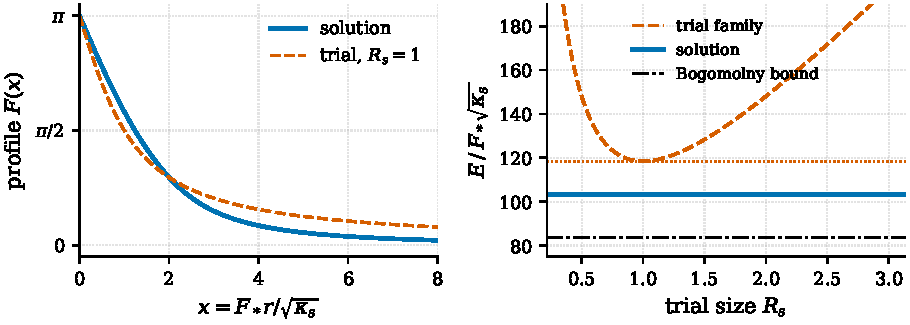
\includegraphics[width=\textwidth]{skyrmion.pdf}
  \caption{The solved defect. \emph{Left:} the hedgehog profile obtained from
    \cref{eq:defects-ode} compared with the trial family at its preferred size;
    the solution has the faster $x^{-2}$ tail. \emph{Right:} energies in units
    of $\Fstar\sqrt{\kaps}$. The trial family (dashed) is minimised at
    $\numSkyrmeTrialMin$, the solution (solid) sits at $\numSkyrmeEnergy$, and
    the Bogomolny bound \cref{eq:defects-bound} (dash-dotted) is
    $\numSkyrmeBound$.}
  \label{fig:skyrmion}
\end{figure}

\paragraph{Limits of this calculation.} A minimum within the hedgehog ansatz is
not a proof of stability against all deformations: that would require the full
Hessian. And the energy of a solution is not a particle mass until the sector
is quantised; the collective coordinates, their moments of inertia, and the
Finkelstein--Rubinstein constraints all enter. What
\cref{eq:defects-solved} establishes is that the localized sector of
\cref{asm:closure} has a concrete, calculable representative with an integer
charge, a finite energy and a preferred size.

\subsection{Why the equation of state is what it is}\label{sec:defects-eos}

Being localized is not by itself enough to be pressureless. For an isotropic
population of objects of mass $m_D$ with distribution $\mathcal F(\mathbf p)$,
%
\begin{equation}\label{eq:defects-eos}
  \rhoD=\int \dd^3p\,E_{\mathbf p}\mathcal F,
  \qquad
  p_D=\frac13\int \dd^3p\,\frac{\mathbf p^2}{E_{\mathbf p}}\mathcal F,
  \qquad
  \frac{p_D}{\rhoD}\simeq\frac{\avg{v^2}}{3}\ \ll1
  \ \text{ iff }\ \abs{\mathbf p}\ll m_D .
\end{equation}
%
So the pressureless assumption is a statement about the momentum distribution
of the products, and formation by absorption could well produce fast objects.
That the conversion is the same process which sets the momentum distribution is
a constraint the model does not currently compute.

Dimensionality matters as much as localization. For a frozen comoving
population of defects of spatial dimension $d$ with energy proportional to
their extent, $\rho\propto a^{d-3}$ and hence $w=-d/3$: point-like relics give
$w=0$, frozen strings $-1/3$, frozen walls $-2/3$. A $U(1)$ vortex in three
dimensions is a string, not a particle, and a string's energy per unit length
being finite does not make an infinite string's energy finite. The texture
above is genuinely three-dimensional and point-like, which is why it is the
representative chosen here.

\subsection{What would be needed for an abundance}\label{sec:defects-abundance}

By \cref{eq:cosmology-survival}, $\rhoD a^3\to\rho_{D,\rm act}+\bfrac\rho_{I,\rm act}$,
so the comoving abundance is fixed by the branching ratio and the initial
data. Converting that into a number density requires the mass $m_D$, which the
background does not constrain, and a viable relic further requires either an
asymmetry or a production rate low enough that annihilation is negligible,
together with a free-streaming length short enough not to erase structure. None
of this is computed here. The topological charge is also not a spin: although
$\pi_4(S^3)=\Int_2$ permits a Finkelstein--Rubinstein quantisation in which the
soliton is a fermion, establishing it requires showing that the $2\pi$ rotation
loop is non-contractible in the configuration space and choosing a
representation of its fundamental group. \Cref{sec:outlook} lists both as open.

\paragraph{What this section establishes.}
A solved, finite-energy, unit-charge configuration with a preferred size, and
the exact conditions under which such a population is pressureless. What it
does not establish is that these objects exist, that they are stable against
general deformations, that they are fermions, or that their relic abundance
matches the observed dark matter.
